
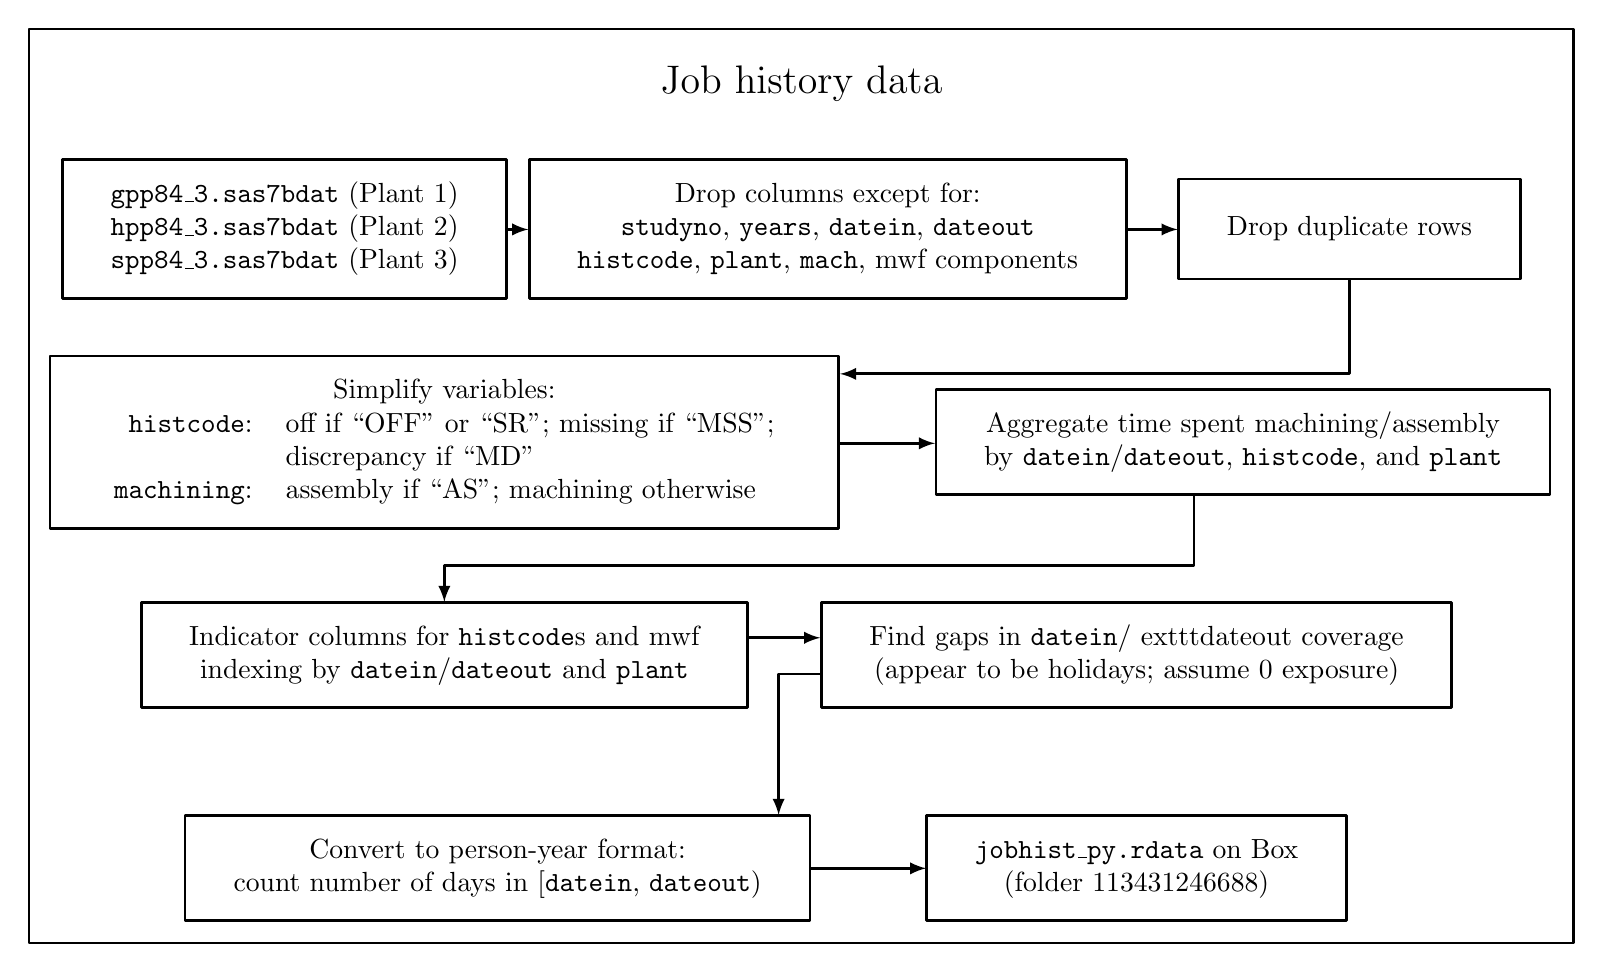
\begin{tikzpicture}[>=latex,line join=bevel,]
  \pgfsetlinewidth{1bp}
%%
\begin{scope}
  \pgfsetstrokecolor{black}
  \definecolor{strokecol}{rgb}{0.0,0.0,0.0}
  \pgfsetstrokecolor{strokecol}
  \draw (0.24bp,0.14bp) -- (0.24bp,329.14bp) -- (556.24bp,329.14bp) -- (556.24bp,0.14bp) -- cycle;
  \draw (278.24bp,309.64bp) node {\Large Job history data};
\end{scope}
  \pgfsetcolor{black}
  % Edge: filter -> drop
  \draw [->] (395.4bp,257.0bp) .. controls (395.4bp,257.0bp) and (403.73bp,257.0bp)  .. (413.73bp,257.0bp);
  % Edge: drop -> simplify
  \draw [->] (475.61bp,238.9bp) .. controls (475.61bp,223.87bp) and (475.61bp,205.0bp)  .. (475.61bp,205.0bp) .. controls (475.61bp,205.0bp) and (302.2bp,205.0bp)  .. (292.2bp,205.0bp);
  % Edge: machining -> histcode
  \draw [->] (419.6bp,161.35bp) .. controls (419.6bp,149.3bp) and (419.6bp,136.0bp)  .. (419.6bp,136.0bp) .. controls (419.6bp,136.0bp) and (149.74bp,136.0bp)  .. (149.74bp,136.0bp) .. controls (149.74bp,136.0bp) and (149.74bp,132.9bp)  .. (149.74bp,122.9bp);
  % Edge: job -> filter
  \draw [->] (172.33bp,257.0bp) .. controls (172.33bp,257.0bp) and (173.09bp,257.0bp)  .. (179.96bp,257.0bp);
  % Edge: simplify -> machining
  \draw [->] (291.82bp,180.0bp) .. controls (291.82bp,180.0bp) and (316.37bp,180.0bp)  .. (326.37bp,180.0bp);
  % Edge: histcode -> cont
  \draw [->] (259.04bp,110.0bp) .. controls (259.04bp,110.0bp) and (275.06bp,110.0bp)  .. (285.06bp,110.0bp);
  % Edge: cont -> clean
  \draw [->] (285.37bp,97.0bp) .. controls (276.03bp,97.0bp) and (270.08bp,97.0bp)  .. (270.08bp,97.0bp) .. controls (270.08bp,97.0bp) and (270.08bp,56.213bp)  .. (270.08bp,46.213bp);
  % Edge: clean -> final
  \draw [->] (281.57bp,27.0bp) .. controls (281.57bp,27.0bp) and (313.2bp,27.0bp)  .. (323.2bp,27.0bp);
  % Node: cont
\begin{scope}
  \definecolor{strokecol}{rgb}{0.0,0.0,0.0}
  \pgfsetstrokecolor{strokecol}
  \draw (512.44bp,122.79bp) -- (285.44bp,122.79bp) -- (285.44bp,84.79bp) -- (512.44bp,84.79bp) -- cycle;
  \draw (398.94bp,103.79bp) node {\begin{tabular}{c} 
						Find gaps in \texttt{datein}/	exttt{dateout} coverage \\						(appear to be holidays; assume 0 exposure)
						\end{tabular}};
\end{scope}
  % Node: drop
\begin{scope}
  \definecolor{strokecol}{rgb}{0.0,0.0,0.0}
  \pgfsetstrokecolor{strokecol}
  \draw (537.11bp,275.14bp) -- (414.11bp,275.14bp) -- (414.11bp,239.14bp) -- (537.11bp,239.14bp) -- cycle;
  \draw (475.61bp,257.14bp) node {\begin{tabular}{c} 
						Drop duplicate rows
						\end{tabular}};
\end{scope}
  % Node: filter
\begin{scope}
  \definecolor{strokecol}{rgb}{0.0,0.0,0.0}
  \pgfsetstrokecolor{strokecol}
  \draw (395.26bp,282.14bp) -- (180.26bp,282.14bp) -- (180.26bp,232.14bp) -- (395.26bp,232.14bp) -- cycle;
  \draw (287.76bp,257.14bp) node {\begin{tabular}{c} 
						Drop columns except for: \\						\texttt{studyno}, \texttt{years}, \texttt{datein}, \texttt{dateout} \\						\texttt{histcode}, \texttt{plant}, \texttt{mach}, mwf components \\						\end{tabular}};
\end{scope}
  % Node: simplify
\begin{scope}
  \definecolor{strokecol}{rgb}{0.0,0.0,0.0}
  \pgfsetstrokecolor{strokecol}
  \draw (291.74bp,211.47bp) -- (7.74bp,211.47bp) -- (7.74bp,149.47bp) -- (291.74bp,149.47bp) -- cycle;
  \draw (149.74bp,180.47bp) node {\begin{tabular}{c} 
						Simplify variables: \\								\begin{tabular}{rl}
								\texttt{histcode}: & off if ``OFF'' or ``SR'';
								missing if ``MSS''; \\								& discrepancy if ``MD'' \\								\texttt{machining}: & assembly if ``AS''; machining otherwise
								\end{tabular}
						\end{tabular}};
\end{scope}
  % Node: job
\begin{scope}
  \definecolor{strokecol}{rgb}{0.0,0.0,0.0}
  \pgfsetstrokecolor{strokecol}
  \draw (172.24bp,282.14bp) -- (12.24bp,282.14bp) -- (12.24bp,232.14bp) -- (172.24bp,232.14bp) -- cycle;
  \draw (92.238bp,257.14bp) node {\begin{tabular}{c} 
						\texttt{gpp84\_3.sas7bdat} (Plant 1) \\						\texttt{hpp84\_3.sas7bdat} (Plant 2) \\						\texttt{spp84\_3.sas7bdat} (Plant 3) \\						\end{tabular}};
\end{scope}
  % Node: machining
\begin{scope}
  \definecolor{strokecol}{rgb}{0.0,0.0,0.0}
  \pgfsetstrokecolor{strokecol}
  \draw (547.77bp,199.47bp) -- (326.77bp,199.47bp) -- (326.77bp,161.47bp) -- (547.77bp,161.47bp) -- cycle;
  \draw (437.27bp,180.47bp) node {\begin{tabular}{c} 
						Aggregate time spent machining/assembly \\						by \texttt{datein}/\texttt{dateout}, \texttt{histcode}, and \texttt{plant}
						\end{tabular}};
\end{scope}
  % Node: clean
\begin{scope}
  \definecolor{strokecol}{rgb}{0.0,0.0,0.0}
  \pgfsetstrokecolor{strokecol}
  \draw (281.41bp,46.12bp) -- (56.41bp,46.12bp) -- (56.41bp,8.12bp) -- (281.41bp,8.12bp) -- cycle;
  \draw (168.91bp,27.118bp) node {\begin{tabular}{c} 
						Convert to person-year format: \\						count number of days in [\texttt{datein}, \texttt{dateout})
						\end{tabular}};
\end{scope}
  % Node: histcode
\begin{scope}
  \definecolor{strokecol}{rgb}{0.0,0.0,0.0}
  \pgfsetstrokecolor{strokecol}
  \draw (258.74bp,122.79bp) -- (40.74bp,122.79bp) -- (40.74bp,84.79bp) -- (258.74bp,84.79bp) -- cycle;
  \draw (149.74bp,103.79bp) node {\begin{tabular}{c} 
						Indicator columns for \texttt{histcode}s and mwf\\						indexing by \texttt{datein}/\texttt{dateout} and \texttt{plant}
						\end{tabular}};
\end{scope}
  % Node: final
\begin{scope}
  \definecolor{strokecol}{rgb}{0.0,0.0,0.0}
  \pgfsetstrokecolor{strokecol}
  \draw (474.44bp,46.12bp) -- (323.44bp,46.12bp) -- (323.44bp,8.12bp) -- (474.44bp,8.12bp) -- cycle;
  \draw (398.94bp,27.118bp) node {\begin{tabular}{c} 
						\texttt{jobhist\_py.rdata} on Box \\						({folder 113431246688})
						\end{tabular}};
\end{scope}
%
\end{tikzpicture}

